%!TEX root=../GaugeCNNTheory.tex


\subsection{میدان‌های کرنل خارج‌قسمتی}
\label{sec:quotient_kernel_fields}


قضیه~\ref{thm:isometry_equivariant_kernel_field_trafos} نشان داد که هم‌متغیری ایزومتری یک تبدیل میدان کرنل، نیازمند نامتغیر بودن میدان کرنل متناظر است.
از آنجایی که قید نامتغیر بودن ایجاب می‌کند که کرنل‌ها بر روی مدارها به اشتراک گذاشته شوند، همانطور که در شکل~\ref{fig:isom_invariant_kernel_field_multiple_orbits} به تصویر کشیده شده است، توصیف ریاضی چنین میدان‌های کرنل نامتغیری زائد است:
یک کرنل منفرد در یک نماینده مدار برای بازسازی میدان کرنل بر روی کل مدار کافی است.
در بخش~\ref{sec:quotient_kernels_stabilizers} ما توصیف‌های معادل و کاهش‌یافته‌ای از میدان‌های کرنل نامتغیر را بر حسب کرنل‌ها بر روی نمایندگان مدار استخراج می‌کنیم.
این کرنل‌های نماینده خود توسط عمل زیرگروه پایدارساز نماینده مدار محدود می‌شوند.
ما یک بالابر (منحصر به فرد) از کرنل‌های نماینده به میدان‌های کرنل نامتغیر پیشنهاد می‌کنیم که یک ایزومورفیسم بین هر دو توصیف برقرار می‌کند.
این ایزومورفیسم بالابر راهی برای پارامترسازی و ساخت تبدیلات میدان کرنل هم‌متغیر نسبت به ایزومتری در یک پیاده‌سازی پیشنهاد می‌کند.
قبل از استخراج این نتایج در بخش~\ref{sec:quotient_kernels_stabilizers}، بخش بعدی~\ref{sec:isom_quotients} چارچوب ریاضی را تنظیم می‌کند.

استخراج‌ها و نتایج این بخش از نظر روحی به نظریه \emph{\lr{CNN}های هدایت‌پذیر در فضاهای همگن} نزدیک است~\cite{Cohen2018-intertwiners,Cohen2019-generaltheory}،
با این حال، ما نتایج آنها را از فضاهای همگن به منیفلدهای عمومی تعمیم می‌دهیم.
هنگامی که به فضاهای همگن $M$ پایبند باشیم، ثابت می‌کنیم که تبدیلات میدان کرنل هم‌متغیر نسبت به ایزومتری با کانولوشن‌های $\GM$ معادل هستند.





\subsubsection{فضاهای خارج‌قسمتی القاشده از ایزومتری}
\label{sec:isom_quotients}


عمل یک گروه تقارن بر روی یک فضا، آن را به مدارهایی افراز می‌کند که به عنوان مجموعه‌هایی از تمام نقاطی که با عمل گروه به هم متصل هستند، تعریف می‌شوند.
فضای چنین مدارهایی، \emph{فضای خارج‌قسمتی} نسبت به این عمل گروهی است.
در ادامه ما فضاهای خارج‌قسمتی ناشی از اعمال یک گروه ایزومتری $\I \leq \IsomGM$ را هم بر روی منیفلد و هم بر روی کلاف‌های تاری مورد بحث قرار خواهیم داد.
این تعاریف بعداً به ما اجازه می‌دهند تا با عمل ایزومتری‌ها بر روی کرنل‌ها، وزن‌ها را بر روی مدارها به اشتراک بگذاریم.



\paragraph{خارج‌قسمت‌های منیفلد:}

هر نقطه $p\in M$ یک \emph{مدار} را ترسیم می‌کند
\begin{align}\label{eq:orbit_Ip}
    \I.p \,:=\, \big\{ \phi(p) \;\big|\; \phi \in\I \,\big\}\ \subseteq\, M \,,
\end{align}
که به عنوان مجموعه تمام نقاطی که با عمل بر روی $p$ با هر ایزومتری در $\I \leq \IsomM$ به دست می‌آیند، تعریف می‌شود.
می‌توان به راحتی بررسی کرد که رابطه «$p$ و $q$ عناصری از یک مدار هستند» یک رابطه هم‌ارزی است (به پاورقی \ref{footnote:equiv_rel} مراجعه کنید) و بنابراین منیفلد را همانطور که در شکل~\ref{fig:isom_egg_quotient_M} به تصویر کشیده شده است، \emph{افراز} می‌کند.
فضای خارج‌قسمتی
\begin{align}\label{eq:quotientspace_IM}
    \IM \, :=\, \big\{ \I.p \,\big|\, p\in M \big\}
\end{align}
نسبت به این رابطه هم‌ارزی، فضای تمام مدارها است، یعنی هر عنصر از $\IM$ متناظر با یک مدار کامل در $M$ است.%
\footnote{%
    ما $\IM$ را به عنوان یک خارج‌قسمت چپ می‌نویسیم زیرا $\I$ از چپ بر روی $M$ عمل می‌کند.
}
\emph{نگاشت خارج‌قسمتی} متناظر
\begin{align}\label{eq:quotientmap_QM}
    \QM: M\to\IM,\ \ p\mapsto \I.p
\end{align}
یک نقطه $p \in M$ را با مدارش $\I.p \in \IM$ شناسایی می‌کند.
برای هر مدار می‌توان یک \emph{نماینده مدار} دلخواه را انتخاب کرد که به طور رسمی توسط یک \emph{مقطع} تعیین می‌شود
\begin{align}\label{eq:section_rM}
    \rM: \IM\to M \quad \textup{به طوری که}\quad \QM\circ\rM = \id_{\IM} \,,
\end{align}
که در آن شرط آخر تضمین می‌کند که نماینده $\rM(\I.p)$ در واقع عنصری از مدار $\I.p$ است.
اغلب به مقاطع پیوسته (یا هموار) علاقه‌مند هستیم، با این حال، اینها به طور کلی وجود ندارند.
بنابراین ما در ادامه \emph{نمی‌خواهیم} که نمایندگان مدار به طور پیوسته انتخاب شوند و در صورت لزوم این نقیصه را بعداً جبران خواهیم کرد.
طبق معمول برای مقاطع، آنها به طور کلی فقط وارون راست نگاشت خارج‌قسمتی هستند اما وارون چپ نیستند، یعنی $\rM\circ\QM \neq \id_M$.
این با یک نمودار جابجایی
\begin{equation}
\begin{tikzcd}[row sep=3em, column sep=4.5em]
      \IM
            \arrow[r, "\rM"]
            \arrow[rr, rounded corners, to path={ 
                  -- ([yshift=-3.ex]\tikztostart.south) 
                  --node[below, pos=.5]{\small$\id_{\IM}$} ([yshift=-3.ex]\tikztotarget.south) 
                  -- (\tikztotarget.south)
                  }]
    & M
            \arrow[r, "\QM"]
    & \IM
\end{tikzcd}
\end{equation}
مشابه با معادله~\eqref{cd:section_proj_idM} و یک نمودار غیرجابجایی
\begin{equation}
\begin{tikzcd}[row sep=3em, column sep=4.5em,
               execute at end picture={
                    \node [] at (-.04, -.46) {$\noncommutative$};
                    }]
      M
            \arrow[r, "\QM"]
            \arrow[rr, rounded corners, to path={ 
                  -- ([yshift=-3.5ex]\tikztostart.south) 
                  --node[below, pos=.5]{\small$\id_M$} ([yshift=-3.5ex]\tikztotarget.south) 
                  -- (\tikztotarget.south)
                  }]
    & \IM
            \arrow[r, "\rM"]
    & M
\end{tikzcd}
\end{equation}
مشابه با معادله~\eqref{cd:section_proj_noncommutative} به تصویر کشیده می‌شود.
تارهای منفرد $\preim{\QM}\mkern-4mu(\I.p) = \I.p \subseteq M$ از نگاشت خارج‌قسمتی $\QM$ توسط خود مدارها داده می‌شوند.
توجه داشته باشید که $M\xrightarrow{\QM}\IM$ به طور کلی یک کلاف تاری \emph{نیست} زیرا مدارها لزوماً با یکدیگر همسان‌ریخت نیستند و بنابراین نمی‌توان آنها را به صورت محلی با یک تار نمونه‌ای مشترک $F$ بدیهی‌سازی کرد، همانطور که در نمودار جابجایی در معادله~\eqref{cd:trivialization_general_intro} لازم است.
بنابراین هر مدار \emph{نوع} خاص خود را دارد که در ارتباط نزدیک با زیرگروه‌های پایدارساز نقاط روی آن مدار خاص است.
\emph{زیرگروه پایدارساز}
\begin{align}
    \Stab{p} \,:=\, \big\{ \xi \in \I \,\big|\, \xi(p)=p \big\} \ \leq\ \I
\end{align}
یک نقطه $p\in M$ به عنوان آن زیرگروهی از گروه ایزومتری که $p$ را ثابت نگه می‌دارد، تعریف می‌شود.
بر حسب زیرگروه پایدارساز، برقرار است که مدار یک نقطه با
\begin{align}
    \I.p \ \cong\ \I/\Stab{p} \,.
\end{align}
شناسایی می‌شود. برای دیدن این ادعا، فرض کنید $f_p: \I \to \I.p,\ \phi \mapsto \phi(p)$ برای یک $p\in M$ و مشاهده کنید که $f_p(\phi\circ\xi) = \phi\circ\xi(p) = \phi(p) = f_p(\phi)$ برای هر $\xi\in\Stab{p}$.
به راحتی می‌توان نشان داد که در واقع $\preim{f_p}\!\! \big(\phi(p)\big) = \phi.\Stab{p}$ یک هَم‌دسته از زیرگروه پایدارساز $p$ است و بنابراین $f_p$ ایزومورفیسم ادعا شده $\I.p \,\cong\, \I/\Stab{p}$ را برقرار می‌کند.

\begin{figure}
    \centering%
    \subcaptionbox{\small نگاشت خارج‌قسمتی و نمایندگان مدار برای $M$.%
        \label{fig:isom_egg_quotient_M}}%
        [.44\linewidth][l]{%
            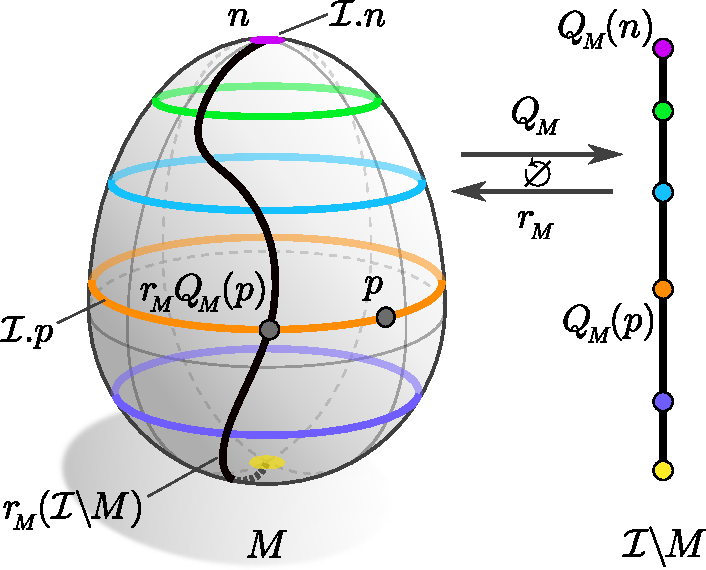
\includegraphics[width=.43\textwidth]{figures/isometry_egg_quotient_M.pdf}%
            \vspace*{1ex}%
        }%
    \hfill%
    \subcaptionbox{\small نگاشت خارج‌قسمتی و نمایندگان مدار برای $\TM$.%
        \label{fig:isom_egg_quotient_TM}}%
        [.5\linewidth][r]{%
            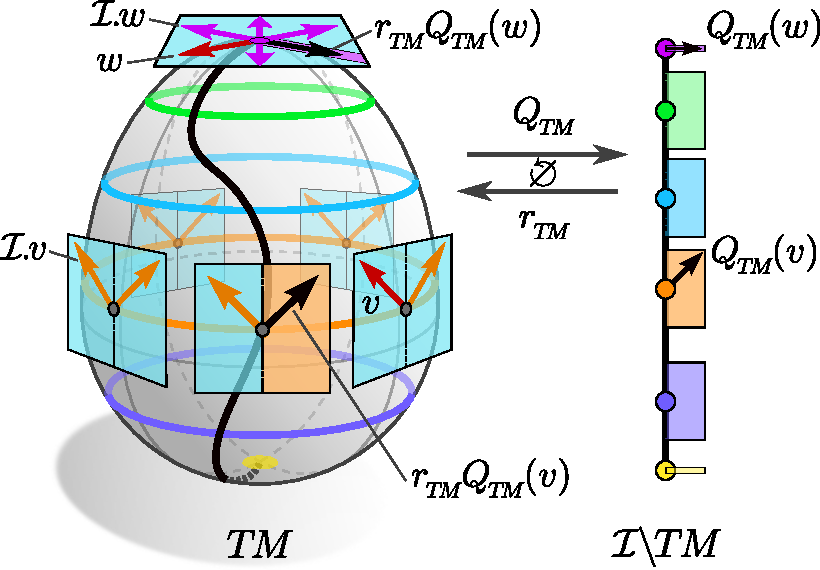
\includegraphics[width=.5\textwidth]{figures/isometry_egg_quotient_TM.pdf}%
            \vspace*{1ex}%
        }%
    \caption{\small%
        نگاشت‌های خارج‌قسمتی $\QM$ و $\QTM$ و نمایندگان مدار (مقاطع) $\rM$ و $\rTM$ برای اعمال گروه ایزومتری $\I=\OO2$ بر روی منیفلد $M$ در شکل~\ref{fig:isom_egg_quotient_M} و بر روی کلاف مماس $\TM$ در شکل~\ref{fig:isom_egg_quotient_TM}.
        توصیف دقیقی از هر دو تصویر در متن اصلی آورده شده است.
    }%
    \label{fig:isom_egg_quotient_main}%
\end{figure}

برای شهودی‌تر کردن این ساختارها، مثال در شکل~\ref{fig:isom_egg_quotient_M} را با $\I \cong \OO2$ در نظر بگیرید.
مدارهای $\I.n = \{n\}$ و $\I.s = \{s\}$ قطب شمال و جنوب فقط نقاطی هستند که توسط $\I$ ثابت می‌شوند.
این با، به عنوان مثال، $\I.n \cong \I/\Stab{n} = \I/\I \cong \{n\}$ موافق است زیرا $\Stab{n}=\I$ با گروه کامل ایزومتری منطبق است.
برای هر نقطه دیگر $p\in M$، مدارهای $\I.p$ دایره هستند.
ما بازتاب‌های $\Stab{p} \cong \Flip$ (بازتاب نسبت به $p$) را به عنوان زیرگروه پایدارساز داریم و بنابراین در واقع دایره $\I/\Stab{p} \cong \OO2/\Flip \cong S^1$ را به عنوان نوع مدار به دست می‌آوریم.
نگاشت خارج‌قسمتی $\QM:M\to\IM$ نقاط $q\in M$ را به مدارهایشان $\QM(q) = \I.q$ در فضای خارج‌قسمتی $\IM$ که در سمت راست نشان داده شده است، می‌فرستد.
از آنجایی که مدارها را می‌توان از قطب شمال تا قطب جنوب پیمود، فضای خارج‌قسمتی $\IM$ توپولوژی یک پاره‌خط را دارد.
مقطع $\rM:\IM\to M$ یک نقطه نماینده $\rM(o) \in M$ را برای هر مدار $o \in \IM$ انتخاب می‌کند.
به طور کلی، این نماینده مدار یک نقطه تصویر شده را بازیابی نمی‌کند.
به عنوان مثال، داریم $\rM\QM(p) \neq p$.
می‌توان مقطع را به عنوان نشاندن فضای خارج‌قسمتی $\IM$ در منیفلد، که به صورت خط سیاه $\rM(\IM)$ از قطب شمال تا قطب جنوب نشان داده شده است، تفسیر کرد.





\paragraph{خارج‌قسمت‌های کلاف:}

از آنجایی که گروه ایزومتری نه تنها بر روی خود منیفلد بلکه از طریق پیش‌ران‌ها بر روی کلاف‌های الحاقی نیز عمل می‌کند، این کلاف‌ها به روشی مشابه به مدارهایی افراز می‌شوند.
برای کلی نگه داشتن بحث، ما در ادامه یک کلاف الحاقی عمومی $E\xrightarrow{\pi_E} M$ را در نظر می‌گیریم که می‌تواند نماینده $\TM$، $\FM$، $\GM$، $\A$ یا $\Hom(\Ain,\Aout)$ باشد.
ما عناصر فضای کل را با $e\in E$ نشان می‌دهیم و فرض می‌کنیم $\dphiE$ پیش‌ران $\phi$ بر روی $E$ باشد همانطور که در بخش~\ref{sec:isom_action_bundles} معرفی شد.
مدار یک عنصر از کلاف سپس به قیاس با معادله~\eqref{eq:orbit_Ip} به صورت زیر داده می‌شود:
\begin{align}\label{eq:bundle_orbit_def}
    \I.e \:=\ \big\{ \dphiE(e) \,\big|\, \phi\in\I \big\}
\end{align}
در حالی که فضای خارج‌قسمتی، که از مدارهای کلاف تشکیل شده است، به طور مشابه با معادله~\eqref{eq:quotientspace_IM} به صورت زیر تعریف می‌شود:
\begin{align}
    \IE \:=\ \big\{ \I.e \,\big|\, e\in E \big\} \,.
\end{align}
مشابه قبل، نگاشت خارج‌قسمتی (کانونی) عناصر کلاف را به مدارشان می‌فرستد:
\begin{align}
    \QE: E\mapsto\IE,\ \ e\mapsto\I.e
\end{align}
ما یک نگاشت تصویر (منحصر به فرد) را تعریف می‌کنیم
\begin{align}\label{eq:quotient_projection_piIE}
    \piIE\!:\, \IE \to \IM, \quad \QE(e) \mapsto \QM \circ \piE(e)
\end{align}
بین خارج‌قسمت‌های کلاف و خارج‌قسمت منیفلد همانطور که در نمودار جابجایی زیر به تصویر کشیده شده است:
\begin{equation}\label{cd:QE_IE}
\begin{tikzcd}[column sep=50pt, row sep=30, font=\normalsize]
    \IE     \arrow[d, "\piIE"']
    &
    E       \arrow[l, "\QE"']
            \arrow[d, "\piE"]
    \\
    \IM
    &
    M       \arrow[l, "\QM"]
\end{tikzcd}
\end{equation}
توجه داشته باشید که تعریف در معادله~\eqref{eq:quotient_projection_piIE} به انتخاب خاص نماینده مدار بستگی ندارد زیرا برای هر $\dphiE(e) \in \QE(e)$ دیگر نتیجه یکسانی به دست می‌آوریم:
$    \QM \circ \piE \circ \dphiE(e)
\,=\,\QM \circ \phi \circ \piE(e)
\,=\,\QM \circ \piE(e) .
$
نمایندگان مدار به طور رسمی توسط یک انتخاب از مقطع تعیین می‌شوند
\begin{align}\label{eq:bundle_quotient_section_def}
    \rE: \IE\to E \quad \textup{به طوری که}\quad \QE\circ\rE = \id_{\IE} \,,
\end{align}
که ما دوباره نمی‌خواهیم پیوسته باشد.
با این حال، برای راحتی، ما می‌خواهیم که نمایندگان مدارهای کلاف بالای نمایندگان $\rM(\IM)$ در فضای پایه قرار گیرند، یعنی برآورده کنند:
\begin{align}\label{eq:bundle_quotient_section_isom}
    \piE \circ \rE \ =\ \rM \circ \piIE
\end{align}
همانطور که در نمودار جابجایی زیر نشان داده شده است:
\begin{equation}
\begin{tikzcd}[column sep=50pt, row sep=30, font=\normalsize]
    \IE     \arrow[d, "\piIE"']
            \arrow[r, "\rE"]
    &
    E       \arrow[d, "\piE"]
    \\
    \IM     \arrow[r, "\rM"']
    &
    M
\end{tikzcd}
\end{equation}


زیرگروه پایدارساز یک عنصر کلاف $e\in E$ به صورت زیر تعریف می‌شود:
\begin{align}
    \Stab{e} \,:=\, \big\{ \xi \in \I \;\big|\; \dxiE e=e \big\} \ \leq\ \Stab{\piE(e)}\ \leq\ \I \,.
\end{align}
این لزوماً یک زیرگروه از زیرگروه پایدارساز $\Stab{\piE(e)}$ نقطه $\piE(e)$ در فضای پایه است، که به راحتی با
$ \ \xi \in \Stab{e}                 \ \Leftrightarrow\ 
    \dxiE e = e                      \ \Rightarrow\ 
    \piE(\dxiE e) = \xi\, \piE(e) = \piE(e) \ \Leftrightarrow\ 
    \xi \in \Stab{\piE(e)} .
$
دیده می‌شود. مانند قبل، رابطه $\I.e \cong \I/\Stab{e}$ برقرار است.


ما مثال خود را از شکل~\ref{fig:isom_egg_quotient_M} با در نظر گرفتن عمل $\I\cong\OO2$ بر روی کلاف مماس $\TM$ تخم‌مرغ $M$ در شکل~\ref{fig:isom_egg_quotient_TM} گسترش می‌دهیم.
مدار (بنفش) یک بردار غیرصفر $0\neq w\in T_nM$ (قرمز) در قطب شمال $n$ یک دایره را در $T_nM$ توصیف می‌کند.
این با $\I.w \cong \I/\Stab{w} \cong \OO2/\Flip \cong S^1$ سازگار است زیرا چنین برداری با بازتاب‌های $\Stab{w} \cong \Flip$ در امتداد محور خود پایدار می‌شود.
مدار $0\in T_nM$ یک نقطه منفرد در $\TM$ است که توسط هر ایزومتری پایدار می‌شود.
هر بردار دیگر $v\in\TpM$ (قرمز)، که در یک فضای مماس در نقطه‌ای $p\in M$ متفاوت از قطب‌ها زندگی می‌کند، با عمل گروه ایزومتری به فضاهای مماس دیگر $\TphipM$ بر روی مدار $\I.p$ از $p$ چرخانده و بازتاب می‌شود.
مدار $\I.v$ (نارنجی) از هر چنین برداری، اگر دقیقاً به سمت شمال یا جنوب اشاره نکند، با یک کپی از بردار به سمت شرق و یک کپی به سمت غرب در هر یک از فضاهای مماس روی $\I.p$ داده می‌شود.
ما برای چنین بردارهایی $\Stab{v}=\{e\}$ داریم و در واقع مدار $\I.v \cong \I/\Stab{v} \cong \OO2/\{e\}$ با $\OO2$ (یا دو دایره) همسان‌ریخت است.
بردارهای $v'\in\TpM$ که دقیقاً به سمت شمال یا جنوب اشاره می‌کنند با بازتاب‌ها روی محوری که تعریف می‌کنند پایدار می‌شوند، یعنی $\Stab{v'} \cong \Flip$.
مدار آنها با یک دایره $\I.v' \cong \I/\Stab{v'} \cong \OO2/\Flip \cong S^1$ همسان‌ریخت است.

نگاشت خارج‌قسمتی $\QTM: \TM \to \ITM$ کلاف مماس را به خارج‌قسمت کلاف $\ITM$ که در نیمه راست شکل~\ref{fig:isom_egg_quotient_TM} نشان داده شده است، تصویر می‌کند.
برای درک ساختار آن، ما تمام موارد کیفی متفاوت را در نظر می‌گیریم:
اولاً، توجه داشته باشید که مدارهای بردارها در قطب‌ها متناظر با دایره‌هایی با شعاع معین هستند، به طوری که مجموعه چنین مدارهایی یک خط $\piIE^{-1}(\I.n) \cong \R^+$ (پرتو صورتی زیر فلش سیاه) را تشکیل می‌دهد.
به طور مشابه، مدارهای بردارها در هر نقطه دیگر $p\in M$ تمام فضاهای مماس $\TphipM$ را روی $\I.p$ در دو بازتاب قطع می‌کنند و بنابراین یک نیم‌صفحه $\piIE^{-1}(\I.p) \cong \R\times\R^+$ (نارنجی) را تشکیل می‌دهند.
مقطع $\rTM: \ITM \to \TM$ هر عنصر خارج‌قسمت کلاف را به یک نماینده در $\TM$ می‌فرستد.
طبق الزام در معادله~\eqref{eq:bundle_quotient_section_isom}، این نمایندگان باید در همان تار روی نمایندگان $\rM(\IM)$ از خارج‌قسمت منیفلد، که به صورت خط سیاه نشان داده شده است، قرار گیرند.
به عنوان مثال، $v\in\TpM$ (قرمز) با نگاشت خارج‌قسمتی به $\QTM(v)\in \ITM$ (سیاه) فرستاده می‌شود.
مقطع $\QTM(v)$ را با $\rTM\QTM(v)$ (همچنین سیاه) نمایش می‌دهد، که عنصری از $T_{\rM\QM(p)}M$ است و به طور کلی با $v$ متفاوت است.



















\subsubsection{میدان‌های کرنل نماینده خارج‌قسمتی و قیود پایدارساز}
\label{sec:quotient_kernels_stabilizers}


برای توجیه ساخت میدان‌های کرنل نماینده خارج‌قسمتی و قیود پایدارساز، فرمول‌بندی صریح‌تر
\begin{align}\label{eq:isom_invariant_kernel_constraint_explicit}
    \dphiHom \!\circ \Kp \circ \dphiTMinv \,=\ \Kphip \qquad \forall\, p\in M,\ \  \phi\in\I \,.
\end{align}
از قید نامتغیر بودن ایزومتری از تعریف~\ref{dfn:isometry_invariant_kernel_fields} را در نظر بگیرید، که با نوشتن معادله~\eqref{eq:kernel_constraint_isom_full_1} برای هر نقطه $p\in M$ به طور جداگانه به دست می‌آید.
این فرمول‌بندی تأکید می‌کند که قید منجر به \emph{اشتراک‌گذاری وزن در امتداد مدارهای منیفلد} $\I.p \in \IM$ می‌شود همانطور که در شکل‌های~\ref{fig:isom_invariant_kernel_field_multiple_orbits} و~\ref{fig:isom_invariant_kernel_field_quotient} به تصویر کشیده شده است.
این ایجاب می‌کند که کرنل $\Kr$ در یک \emph{نقطه نماینده دلخواه} $r = \rM(o)$ از هر مدار $o = \I.r$ به طور کامل میدان کرنل را در بقیه مدار، یعنی در تمام نقاط $\phi(r)$ که $\phi\in\I$ است، مشخص می‌کند.
کرنل $\Kr$ در نقطه نماینده $r$ خود توسط زیرگروه پایدارساز $r$ محدود می‌شود:
\begin{align}\label{eq:stab_constraint_teaser}
    \dxiHom \!\circ \Kr \circ \dxiTMinv \,=\ \Kr \qquad \forall\, \xi\in\Stab{r} \,.
\end{align}
این ایجاب می‌کند که هر میدان کرنل نامتغیر نسبت به ایزومتری را می‌توان بر حسب یک میدان از کرنل‌ها بر روی نمایندگان مدار منیفلد $r \in \rM(\IM)$ که معادله~\eqref{eq:stab_constraint_teaser} را برآورده می‌کنند، پارامترسازی کرد.

در صورتی که زیرگروه پایدارساز در $r$ غیربدیهی باشد، قید پایدارساز در معادله~\eqref{eq:stab_constraint_teaser} تقارن‌های بیشتری را برای خود کرنل $\Kr$ در $r$ ایجاب می‌کند.
به عنوان مثال، در مثال شکل~\ref{fig:isom_invariant_kernel_field_quotient} زیرگروه پایدارساز ${\Stab{r} \cong \Flip}$ بر روی مدار برجسته شده وجود دارد که تقارن بازتابی کرنل‌ها را اعمال می‌کند.
چنین تقارن‌های پایدارسازی امکان فشرده‌سازی بیشتر توصیف میدان‌های کرنل نامتغیر نسبت به ایزومتری را فراهم می‌کند:
مشخص می‌شود که دانستن مقادیر $\K(w)$ میدان کرنل فقط بر روی نمایندگان خارج‌قسمتی کلاف مماس $w \in \rTM(\ITM) \subseteq \TM$ کافی است.
در شکل~\ref{fig:isom_invariant_kernel_field_quotient} این متناظر با دانستن مقادیر کرنل بر روی نیم‌فضای برجسته شده با رنگ نارنجی است، که از آن می‌توان میدان کامل بر روی مدار را با تقارن‌های بازتابی و دورانی در $\I\cong\OO2$ بازسازی کرد.



قضیه~\ref{thm:tangent_quotient_repr_kernel_fields} در زیر ادعای اخیر را دقیق می‌کند با اثبات اینکه فضای $\KIfull$ از میدان‌های کرنل نامتغیر نسبت به ایزومتری با یک فضای $\KIquot$ از میدان‌های کرنل بر روی نمایندگان مدار کلاف مماس $\rTM(\ITM)$ ایزومورف است.
$\KIquot$ با قیود حداکثر کاهش‌یافته مشخص می‌شود و بنابراین میدان‌های کرنل را در $\KIfull$ به روشی غیرزائد کدگذاری می‌کند.
در قضیه~\ref{thm:manifold_quotient_repr_kernel_fields} ما یک فضای ایزومورف سوم $\KIquothat$ را فرمول‌بندی می‌کنیم که به طور معادل میدان‌های کرنل نامتغیر نسبت به ایزومتری را بر حسب کرنل‌های $\Kr$ با قید زیرگروه پایدارساز از معادله~\eqref{eq:stab_constraint_teaser} توصیف می‌کند.
درحالی‌که فرمول‌بندی میدان‌های کرنل نامتغیر نسبت به ایزومتری بر حسب $\KIquothat$ شامل قیود قوی‌تری نسبت به فرمول‌بندی بر حسب $\KIquot$ است، ممکن است برای پیاده‌سازی‌ها راحت‌تر باشد، زیرا کرنل‌ها را بر روی فضاهای مماس کامل به جای کرنل‌ها بر روی خارج‌قسمت‌های فضاهای مماس توصیف می‌کند.

\begin{SCfigure}
    \centering
    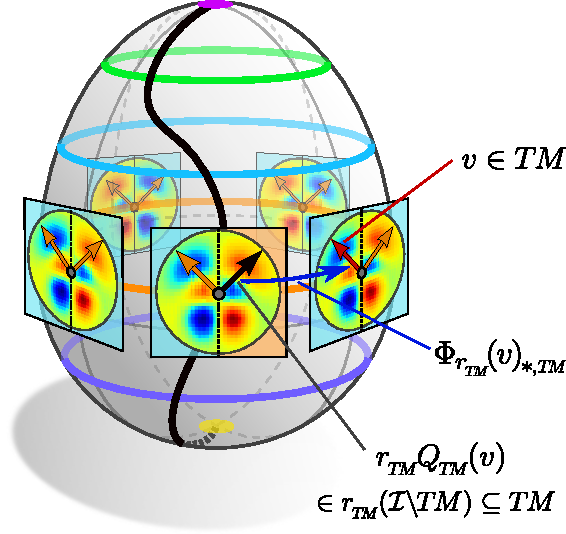
\includegraphics[width=.51\columnwidth]{figures/isometry_egg_quotient_kernel.pdf}
    \captionsetup{width=1.\textwidth}
    \hfill
    \caption{\small
        نمایش تصویری یک میدان کرنل نامتغیر نسبت به ایزومتری، تعریف~\ref{dfn:isometry_invariant_kernel_fields}، و بازسازی کامل آن فقط از کرنل‌ها بر روی نمایندگان خارج‌قسمتی.
        برخلاف شکل~\ref{fig:isom_invariant_kernel_field_multiple_orbits}، ما در اینجا یک گروه ایزومتری $\I = \OO2$ را به جای $\SO2$ فرض می‌کنیم.
        بنابراین کرنل‌های به تصویر کشیده شده دارای تقارن بازتابی هستند که توسط زیرگروه‌های پایدارساز $\Stab{p} \!\cong\! \Flip$ از نقاط روی مدار $\I.\piTM(v)$ اعمال می‌شود.
        به دلیل تقارنش، میدان کرنل کامل $\K: \TM\to \Hom(\Ain,\Aout)$ را می‌توان از محدودیت آن به نماینده خارج‌قسمتی کلاف $\rTM(\ITM) \subseteq \TM$ بازسازی کرد؛ به قضیه~\ref{thm:tangent_quotient_repr_kernel_fields} مراجعه کنید.
        به عنوان مثال، کرنل‌های نشان داده شده به طور کامل توسط کرنل جزئی روی نیم‌فضای نارنجی تعیین می‌شوند.
        بازسازی در $v\in \TM$ با ارزیابی کرنل نماینده خارج‌قسمتی در $\rTM\QTM(v) \in \rTM(\ITM)$ و پیش‌ران کردن کرنل از طریق ایزومتری بازسازی $\PhirNoArg(v) \in \I$، که در معادله~\eqref{eq:reconstruction_isometry} تعریف شده است، به $v$ انجام می‌شود.
        ما می‌خواهیم ذکر کنیم که کرنل‌های \emph{پادمتقارن} به تصویر کشیده شده هنگام نگاشت بین میدان‌های ویژگی با پاریته زوج و فرد حاصل می‌شوند، در حالی که کرنل‌ها بین میدان‌های ویژگی با پاریته یکسان متقارن خواهند بود.
        }
    \label{fig:isom_invariant_kernel_field_quotient}
\end{SCfigure}



\paragraph{ایزومتری‌های بازسازی:}
برای بازسازی میدان‌های کرنل نامتغیر کامل در $\KIfull$ از کرنل‌های منفرد بر روی نمایندگان مدار، کرنل‌های نماینده باید با اعمال پیش‌ران کرنل در معادله~\eqref{eq:isom_invariant_kernel_constraint_explicit} با $p=r$ ثابت برای نقاط نماینده انتخاب‌شده، بر روی کل منیفلد توزیع شوند.
برای بازسازی کرنل در یک نقطه $q\in M$، این به یک ایزومتری $\phi$ نیاز دارد که نماینده مدار $\rM\QM(q) \in \rM(\IM) \subseteq M$ را به $q\in M$ بازگرداند، یعنی $\phi\big(\rM\QM(q)\big) = q$ را برآورده کند.
برای دقیق‌تر کردن این، به یاد بیاورید که میدان‌های کرنل $\K: \TM\to \Hom(\Ain,\Aout)$ به عنوان نگاشت‌هایی با دامنه $\TM$ تعریف می‌شوند، که علاوه بر موقعیتشان، \emph{ترازهای کرنل} را نیز کدگذاری می‌کنند.
بنابراین ما باید ایزومتری‌های خاص‌تری را در نظر بگیریم که نمایندگان مدار کلاف مماس $\rTM\QTM(v) \in \rTM(\ITM) \subseteq \TM$ را به بردارها $v \in \TM$ بازمی‌گردانند.
این \emph{ایزومتری‌های بازسازی} به صورت زیر تعریف می‌شوند:%
\footnote{
    از آنجایی که مقاطع $\rTM$ به طور کلی پیوسته نیستند، $\PhirNoArg$ نیز به طور کلی نمی‌تواند پیوسته خواسته شود.
}
\begin{align}\label{eq:reconstruction_isometry}
    \PhirNoArg: \TM \to \I \quad\textup{به طوری که}\quad \dPhirTM{v}\, \rTM\mkern1mu \QTM(v) = v \quad \forall\, v\in \TM
\end{align}
ما توصیه می‌کنیم برای به دست آوردن شهودی از ایزومتری‌های بازسازی به شکل~\ref{fig:isom_invariant_kernel_field_quotient} مراجعه کنید:
از نظر گرافیکی، $\Phir{v}$ به عنوان \emph{هر} ایزومتری تعریف می‌شود که بردار سیاه $\rTM\QTM(v)$ را روی مدار نارنجی $\I.v$ به بردار قرمز $v$ روی همان مدار بازمی‌گرداند.
توجه داشته باشید که $\PhirNoArg$ تنها تا زیرگروه‌های پایدارساز نمایندگان مدار منحصر به فرد است زیرا برای هر $\xi\in \Stab{\rTM\QTM(v)}$ نتیجه می‌شود که $\Phir{v} \xi$ نیز قید تعریف‌کننده در معادله~\eqref{eq:reconstruction_isometry} را برآورده می‌کند:%
\footnote{\label{footnote:ambiguity_reconstruction_isometry_persian}:%
    علاوه بر این، قید تعریف‌کننده بر روی $\PhirNoArg$ هنگام ضرب \emph{چپ} $\Phir{v}$ با هر $\zeta\in\Stab{v}$ برآورده می‌شود.
    این، با این حال، هیچ درجه آزادی جدیدی اضافه نمی‌کند زیرا $\Stab{v} \cong \Stab{\rTM\QTM(v)}$ و
    $\zeta\,\Phir{v} = \Phir{v} \big[\Phir{v}^{-1} \zeta \Phir{v}\big] =: \Phir{v} \widetilde{\zeta}$
    با $\widetilde{\zeta} \in \Stab{\rTM\QTM(v)}$.
}
$\big[ \Phir{v}\, \xi\, \big]_{\!*,\scalebox{.58}{$T\mkern-1.5muM$}}\mkern2mu \rTM\QTM(v) = \dPhirTM{v}\, \rTM\QTM(v) = v$.
نشان داده می‌شود که تمام ساختارهای بعدی از این ابهام مستقل هستند.
عمل ایزومتری‌های بازسازی بر روی فضای پایه $M$ با اعمال تصویر کلاف مماس بر هر دو طرف قید تعریف‌کننده در معادله~\eqref{eq:reconstruction_isometry} به دست می‌آید:
\begin{alignat}{3}\label{eq:reconstruction_isometry_basespace}
    \qquad\qquad\qquad
    \piTM(v)
    \ &=\ \piTM \dPhirTM{v}\, \rTM\, \QTM(v)
        \qquad\quad && \big( \textup{\small تعریف $\PhirNoArg\,$, معادلۀ~\eqref{eq:reconstruction_isometry} } \big) \notag \\
    \ &=\ \Phir{v}\, \piTM\, \rTM\, \QTM(v)
        \qquad\quad && \big( \textup{\small پیش‌ران یک نگاشت کلاف است، معادلۀ~\eqref{eq:pushfwd_bundle_automorphism} } \big) \notag \\
    \ &=\ \Phir{v}\, \rM\, \piITM\, \QTM(v)
        \qquad\quad && \big( \textup{\small تعریف مقاطع کلاف، معادلۀ~\eqref{eq:bundle_quotient_section_isom} } \big) \notag \\
    \ &=\ \Phir{v}\, \rM\, \QM\,  \piTM(v)
        \qquad\quad && \big( \textup{\small تعریف $\piIE\,$, معادلۀ~\eqref{cd:QE_IE} } \big)
\end{alignat}
یک خلاصه بصری از ویژگی‌های $\PhirNoArg$ یعنی اعمال آن بر روی $\TM$ و $M$ در نمودار جابجایی زیر آورده شده است:
\begin{equation}
    \begin{tikzcd}[row sep=3.5em, column sep=6em]
        % ROW 1
        \TM
            \arrow[d, "\piTM"']
            \arrow[r, "\PhirNoArg \,\times\ \rTM \mkern-2mu\circ\mkern-2mu \QTM"]
            \arrow[rr, rounded corners, to path={ 
                    -- ([yshift=+5.5ex]\tikztostart.north) 
                    --node[above, pos=.5]{\small$\id_{\TM}$} ([yshift=+5.5ex]\tikztotarget.north) 
                    -- (\tikztotarget.north)
                    }]
        &[10ex]
        \I \times \rTM(\ITM)
            \arrow[r, "\ev"]
            \arrow[d, "\id_{\I} \times \piTM"']
        & \TM
            \arrow[d, "\piTM"]
        \\
        % ROW 2
          M
            \arrow[rr, rounded corners, to path={ 
                    -- ([yshift=-5.5ex]\tikztostart.south) 
                    --node[below, pos=.5]{\small$\id_M$} ([yshift=-5.5ex]\tikztotarget.south) 
                    -- (\tikztotarget.south)
                    }]
        &[10ex] \I \times \rM(\IM)
            \arrow[r, pos=.52, "\ev"']
        & M
    \end{tikzcd}
    \quad
\end{equation}
که در آن \emph{نگاشت‌های ارزیابی} $\ev$ با استفاده بیش از حد از نمادگذاری، به ترتیب با $\ev: \I\times  M \to  M,\ (\phi,p) \mapsto \phi(p)$ و $\ev: \I\times \TM \to \TM,\ (\phi,v) \mapsto \dphiTM(v)$ داده می‌شوند.




\paragraph{میدان‌های کرنل نماینده خارج‌قسمتی:}
همانطور که در بالا استدلال شد، تقارن‌های موجود در یک میدان ویژگی \mbox{نامتغیر} نسبت به \mbox{ایزومتری} $\K \in \KIfull$ باید امکان بازسازی کامل آن را از محدودیتش ${\Krestr: \rTM(\ITM) \to \rHom(\IHom)}$ به نمایندگان مدار کلاف مماس $\rTM(\ITM) \subseteq \TM$ فراهم کنند.%
\footnote{
    در ادامه ممکن است $\Hom(\Ain,\Aout)$ و $\I\backslash \Hom(\Ain,\Aout)$ را به ترتیب با $\Hom$ و $\IHom$ به اختصار بنویسیم.
}
برای ساخت یک \emph{بالابر} (منحصر به فرد) $\Lambda$ که $\K = \Lambda(\Krestr)$ را از $\Krestr$ بازیابی می‌کند، ما بردارهای مماس $v$ را در دامنه $\K$ از طریق ایزومتری بازسازی $\PhirNoArg$ از معادله~\eqref{eq:reconstruction_isometry} بسط می‌دهیم و از نامتغیر بودن (هم‌متغیر بودن) میدان کرنل در معادله~\eqref{eq:kernel_constraint_isom_full_1} استفاده می‌کنیم.
این منجر به موارد زیر می‌شود:
\begin{align}\label{eq:lambda_construction}
    \K(v)
    \ &=\,\ \K\; \dPhirTM{v}\; \rTM\, \QTM (v) \notag \\
    \ &=\,\ \dPhirHom{v}\, \K\; \rTM\, \QTM (v) \notag \\
    \ &=\,\ \dPhirHom{v}\, \Krestr\, \rTM\, \QTM (v) \notag \\
    \ &=:\  \pig[ \Lambda\big(\Krestr\big) \pig] (v)
\end{align}
توجه داشته باشید که این ساختار با وجود ابهام $\PhirNoArg$ نسبت به ضرب راست با عناصر در $\Stab{\rTM\QTM(v)}$ خوش‌تعریف است.
این به راحتی با مشاهده اینکه برای هر $w \in \TM$ هر $\xi \in \Stab{w}$ و هر $\K \in \KIfull$ داریم $\dxiHom \K(w) = \K(\dxiTM w) = \K(w)$ که ایجاب می‌کند $\Stab{\K(w)} \geq \Stab{w}$ و بنابراین نتیجه نهایی به انتخاب خاص $\PhirNoArg$ مبهم بستگی ندارد، دیده می‌شود.


از آنجایی که بالابر $\Lambda$ میدان‌های کرنل نامتغیر را از محدودیت آنها به نمایندگان مدار کلاف مماس بازیابی می‌کند، می‌توان آن را به عنوان نگاشت \emph{معکوس} محدودیت (از میدان‌های کرنل نامتغیر) در نظر گرفت.
این دیدگاه ایجاب می‌کند که بالابر یک \emph{ایزومورفیسم} $\Lambda: \KIquot \to \KIfull$ بین تصویر محدودیت $\KIquot$ که هنوز باید آن را مشخص کنیم و $\KIfull$ برقرار می‌کند:
\begin{equation}
    \begin{tikzcd}[row sep=3.5em, column sep=12.em]
        \KIquot
            \arrow[r, bend left=8, shift left=2pt, "\Lambda"]
        &
        \KIfull
            \arrow[l, bend left=8, shift left=2pt, "\Lambda^{-1} = (\,\cdot\,)|_{\rTM(\ITM)}"]
    \end{tikzcd}
\end{equation}

برای مشخص کردن فضای $\KIquot$ که $\Lambda$ را به یک ایزومورفیسم تبدیل می‌کند، کافی است ویژگی‌های میدان‌های محدود شده $\Q := \Krestr \in \KIquot$ را برای $\K \in \KIfull$ فهرست کنیم:
\begin{itemize}[leftmargin=0.6cm]

\item[{\rule[2.2pt]{2pt}{2pt}}]
اول از همه، از آنجایی که $\Lambda^{-1}$ با محدودیت دامنه به $\rTM(\ITM)$ داده می‌شود، واضح است که هر $\Q \in \KIquot$ باید به شکل $\Q: \rTM(\ITM) \to \rHom(\IHom)$ باشد.

\item[{\rule[2.2pt]{2pt}{2pt}}]
دوم، ویژگی میدان‌های کرنل برای اینکه \lr{M}-مورفیسم‌های کلاف باشند، تحت محدودیت $\Lambda^{-1}$ به این الزام برای $\Q$ ترجمه می‌شود که $\piHom\circ\Q(w) = \piTM(w)$ را برای هر $w\in \rTM(\ITM)$ برآورده کند.

\item[{\rule[2.2pt]{2pt}{2pt}}]
سوم، $\Q$ باید \emph{قید پایدارساز (برداری)} $\dxiHom \Q(w) = \Q(w)$ را برای هر بردار نماینده $w \mkern-2mu\in\mkern-1mu \rTM(\ITM)$ و هر $\xi \mkern-1mu\in\mkern-1mu \Stab{w}$ برآورده کند.
این الزام باقیمانده‌ای از قید نامتغیر بودن در معادله~\eqref{eq:kernel_constraint_isom_full_1} است که پس از محدودیت باقی می‌ماند.
\\
این را می‌توان با در نظر گرفتن قید کامل $\dphiHom \Q\, \dphiTMinv(w) = \Q(w)$ برای هر $w \in \rTM(\ITM)$ و هر ایزومتری $\phi\in\I$ که علاوه بر این برآورده می‌کند $\dphiTM(w) \in \rTM(\ITM)$، یعنی پیش‌ران $\dphiTM(w)$ در دامنه محدود شده $\Q$ باقی می‌ماند، استنتاج کرد.
توجه داشته باشید که $\dphiTM(w) \in \I.w$ و اینکه $\rTM(\ITM)$ هر مدار را دقیقاً یک بار قطع می‌کند.
این ایجاب می‌کند که $\I.w \cap \rTM(\ITM) = \{w\}$ به طوری که $\phi\in\I$ باید $\dphiTM(w)=w$ را برآورده کند، یعنی $\phi\in \Stab{w}$.
قید پایدارساز (برداری) ادعا شده از این ملاحظات نتیجه می‌شود.
\\
برای شهود به شکل~\ref{fig:isom_invariant_kernel_field_quotient} بازمی‌گردیم که در آن بردار نماینده سیاه $w = \rTM\QTM(v)$ فقط با ایزومتری بدیهی $\xi=\{e\}$ پایدار می‌شود، که ایجاب می‌کند مقدار متناظر $\Q$ بدون قید باشد.
بردارهای $w' \in \rTM(\ITM)$ که دقیقاً به سمت شمال یا جنوب اشاره می‌کنند، یعنی روی محور بازتابی خط‌چین قرار دارند، با بازتاب‌ها در $\Stab{w'}\cong\Flip$ پایدار می‌شوند، که قیدی را بر روی مقادیر کرنل متناظر ایجاب می‌کند.%
\footnote{
    قید دقیق به عمل $\dxiHom$ بر روی $\Hom(\Ain,\Aout)$ بستگی دارد، که به $\rhoHom$ و بنابراین به $\rhoin$ و $\rhoout$ بستگی دارد.
    کرنل به تصویر کشیده شده در شکل~\eqref{fig:isom_invariant_kernel_field_quotient} متناظر با $\rhoHom$ به عنوان نمایش بازتاب-علامت (پاریته فرد) گروه بازتابی خواهد بود، که کرنل‌های پادمتقارن را اعمال می‌کند.
    پادمتقارن بودن مستلزم آن است که $\Q$ به $\Q(w') = -\Q(w') = 0$ برای $w'$ روی محور بازتابی محدود شود؛ مقایسه کنید با جدول~\ref{tab:reflection_steerable_kernels}
}

\item[{\rule[2.4pt]{2pt}{2pt}}]
به عنوان آخرین الزام، $\Q$ باید به یک میدان کرنل \emph{هموار} بالابر شود، یعنی $\Lambda(\Q)$ باید هموار باشد.
متأسفانه، همواری (یا حتی پیوستگی) $\Lambda(\Q)$ به طور خودکار از همواری (پیوستگی) $\Q$ نتیجه نمی‌شود زیرا $\Lambda$ بر حسب $\rTM$ و $\PhirNoArg$ تعریف می‌شود، که به طور کلی نمی‌توان آنها را هموار (پیوسته) خواست.

\end{itemize}


قبل از خلاصه کردن و اثبات دقیق این ادعاها در قضیه~\ref{thm:tangent_quotient_repr_kernel_fields} در زیر، ما یک نمای کلی بصری از رابطه بین $\Q = \Krestr \in \KIquot$ و بالابر آن $\K = \Lambda(\Q) \in \KIfull$ را در قالب نمودارهای جابجایی ارائه می‌دهیم:
\begin{equation}
    \begin{tikzcd}[row sep=3.5em, column sep=6em]
        % ROW 1
        \TM
            \arrow[r, "\PhirNoArg \,\times\ \Q \mkern-2mu\circ\mkern-2mu \rTM \mkern-2mu\circ\mkern-2mu \QTM"']
            \arrow[rr, rounded corners, to path={ 
                    -- ([yshift=+3.5ex]\tikztostart.north) 
                    --node[above, pos=.5]{\small$\K = \Lambda(\Q)$} ([yshift=+3.5ex]\tikztotarget.north) 
                    -- (\tikztotarget.north)
                    }]
        &[10ex]
        \I \times \rHom(\IHom)
            \arrow[r, "\ev"']
        & \Hom
    \end{tikzcd}
    \qquad
\end{equation}
و
\begin{equation}
    \begin{tikzcd}[row sep=5em, column sep=7.5em]
        % ROW 1
        \TM
            \arrow[rd, pos=.6, "\rTM\circ\QTM"]
            \arrow[rrddd, "\piTM"']
            \arrow[rrrr, "\K = \Lambda(\Q)"]
        & &[-7em] &[-7em] &
        \Hom
            \arrow[ld, pos=.6, "\rHom\circ\QHom"']
            \arrow[llddd, "\piHom"]
        \\[-1em]
        % ROW 2
        & \rTM(\ITM)
            \arrow[rr, "\Q"]
            \arrow[rd, start anchor={[xshift=-1ex]}, "\piTM"']
        & &
        \mkern-3mu
        \rHom(\IHom)
            \arrow[ld, "\piHom"]
        \\
        % ROW 3
        & &
        \rM(\IM)
        \\
        % ROW 4
        & &
        M
            \arrow[u, pos=.6, "\rM \!\circ\mkern-1mu \QM"' description]
    \end{tikzcd}
\end{equation}
در نمودار آخر، جابجایی‌پذیری مربع بالایی با جایگذاری تعریف بالابر به دست می‌آید، که نتیجه می‌دهد
$\rHom\QHom \Lambda(\Q) = \rHom\QHom \dPhirHom{v} \Q\, \rTM\QTM = \Q\, \rTM\QTM$.
جابجایی‌پذیری مربع‌های پایین چپ و راست از معادلات~\ref{eq:bundle_quotient_section_isom} و~\ref{eq:quotient_projection_piIE} نتیجه می‌شود.


\begin{thm}[میدان‌های کرنل نماینده خارج‌قسمتی مماس]
\label{thm:tangent_quotient_repr_kernel_fields}
    فضای میدان‌های کرنل نامتغیر نسبت به ایزومتری $\KIfull$ از تعریف~\ref{dfn:isometry_invariant_kernel_fields} با فضای $\KIquot$ از میدان‌های کرنل با قید زیرگروه پایدارساز (برداری) بر روی نمایندگان خارج‌قسمتی کلاف مماس، که به صورت زیر تعریف می‌شود، ایزومورف است:%
    \footnote{
        این تعریف از $\KIquot$ در وابستگی دوری با تعریف $\Lambda$ در معادله~\eqref{eq:lifting_isomorphism_lambda} است.
        این را می‌توان با هزینه ۱) تعریف فضاهای $\widetilde{\KIquot}$ و $\widetilde{\KIfull}$ بدون الزامات همواری، که بر حسب آنها ۲) $\widetilde{\Lambda}: \widetilde{\KIquot} \to \widetilde{\KIfull}$ را می‌توان تعریف کرد، که ۳) اجازه می‌دهد الزامات همواری را در $\KIquot$ بر حسب $\widetilde{\Lambda}$ بخواهیم، اجتناب کرد.
    }
    \begin{align}\label{eq:KIquot_def}
        \KIquot :=\,
            \Big\{ \Q \mkern-2mu: \rTM(\ITM) \to \rHom(\IHom) \,\Big|\:& 
            \piHom \mkern-5mu\circ\mkern-1mu \Q = \piTM,\quad
            \Lambda(\Q)\ \textup{هموار}, \\ &
            \dxiHom \Q(w) = \Q(w) \ \ \ \forall\; w \mkern-2mu\in\mkern-1mu \rTM(\ITM),\ \xi \mkern-1mu\in\mkern-1mu \Stab{w}
            \!\Big\} \notag
    \end{align}
    \emph{ایزومورفیسم بالابر} (منحصر به فرد) $\Lambda: \KIquot \to \KIfull$ بین هر دو فضا در اینجا به صورت زیر داده می‌شود:
    \begin{align}\label{eq:lifting_isomorphism_lambda}
        \Lambda(\Q): \TM \to \Hom(\Ain,\Aout),\ \ \ 
        v \mapsto \big[ \Lambda(\Q) \big](v) \,:=\, \dPhirHom{v} \Q\; \rTM \QTM(v) \,.
    \end{align}
    معکوس آن $\Lambda^{-1}: \KIfull \to \KIquot$ با محدودیت میدان‌های کرنل نامتغیر به نمایندگان خارج‌قسمتی کلاف $\rTM(\ITM) \subseteq \TM$ داده می‌شود:
    \begin{align}\label{eq:lifting_isomorphism_lambda_inv}
        \Lambda^{-1}(\K): \rTM(\ITM) \to \rHom(\IHom),\ \ \ 
        w \mapsto \big[ \Lambda^{-1}(\K) \big](w) \,:=\, \Krestr(w)
    \end{align}
\end{thm}
\begin{proof}
    برای اثبات اینکه $\Lambda: \KIquot \to \KIfull$ یک ایزومورفیسم است، باید نشان دهیم که
    \textit{1)} $\Lambda^{-1}$ در واقع معکوس $\Lambda$ است، که
    \textit{2)} ویژگی‌های تعریف‌کننده $\KIfull$ و $\KIquot$ پس از بالابر و محدود کردن برآورده می‌شوند و اینکه
    \textit{3)} ساختارها به انتخاب‌های دلخواه بستگی ندارند.
    برای اینکه این بخش بیش از حد سنگین نشود، ما اثبات کامل را به پیوست~\ref{apx:lifting_iso_proof} موکول می‌کنیم.
    مراحل منفرد اثبات در زیر فهرست شده‌اند:
\begin{itemize}[leftmargin=1.25cm]
	\farsiitem{۱آ} $\Lambda \circ \Lambda^{-1} = \id_{\KIfull}$،
	یعنی، $\Lambda^{-1}$ یک وارون راست از $\Lambda$ است
	\farsiitem{۱ب} $\Lambda^{-1} \circ \Lambda = \id_{\KIquot}$،
	یعنی، $\Lambda^{-1}$ یک وارون چپ از $\Lambda$ است
	\farsiitem{۲آ} $\piHom \mkern-5mu\circ\mkern-2mu \Lambda(\Q) = \piTM$ برای هر $\Q \in \KIquot$،
	یعنی، بالابر $\Lambda(\Q)$ یک \lr{M}-مورفیسم کلاف است
	\farsiitem{۲ب} ${\piHom \mkern-5mu\circ\mkern-2mu \Lambda^{-1}(\K) = \piTM}$ برای هر $\K \in \KIfull$
	\farsiitem{۲ج} $\dphiHom \Lambda(\Q)\, \dphiTMinv = \Lambda(\Q)\ \ \forall \phi \in \I$،
	یعنی، $\Lambda(\Q)$ قید کامل نامتغیر بودن (هم‌متغیر بودن) ایزومتری را برآورده می‌کند
	\farsiitem{۲د} $\dxiHom \big[\Lambda^{-1}(\K)\big](w) = \big[\Lambda^{-1}(\K)\big](w) \ \ \
	\forall\; w \mkern-2mu\in\mkern-1mu \rTM(\ITM),\ \xi \mkern-1mu\in\mkern-1mu \Stab{w}$، 
	یعنی، $\Lambda^{-1}(\K)$ قید پایدارساز را برآورده می‌کند
	\farsiitem{۳} تمام ساختارها و اثبات‌ها از انتخاب خاص $\PhirNoArg$ مستقل هستند
\end{itemize}
    همواری میدان‌های کرنل نماینده خارج‌قسمتی بالابر شده بنا به تعریف برقرار است.
\end{proof}
اختیاری بودن در انتخاب مقطع $\rTM$ به میدان‌های کرنل خارج‌قسمتی متفاوت اما ایزومورف، که بر روی نمایندگان خارج‌قسمتی کلاف مختلف بیان شده‌اند، اجازه می‌دهد.


به جای محدود کردن حداکثری میدان کرنل به نمایندگان مدار کلاف در $\rTM(\IM)$، می‌توان توصیف را فقط به $\piTM^{-1}\big( \rM(\IM) \big)$ محدود کرد، یعنی به \emph{فضاهای مماس کامل} $T_rM$ برای هر $r\in \rM(\IM)$.
در شکل~\eqref{fig:isom_invariant_kernel_field_quotient}، این متناظر با مدل‌سازی کرنل (متقارن بازتابی) بر روی کل فضای مماس نشان داده شده در جلو به جای فقط یک نیمه است.
الزامات بر روی چنین کرنل‌های محدود شده‌ای را می‌توان با دنبال کردن همان منطق قبلی استخراج کرد و به قید در معادله~\eqref{eq:stab_constraint_teaser} منجر می‌شود.
ما یک قضیه مشابه با قضیه~\eqref{thm:tangent_quotient_repr_kernel_fields} به دست می‌آوریم:


\begin{thm}[میدان‌های کرنل نماینده خارج‌قسمتی منیفلد]
\label{thm:manifold_quotient_repr_kernel_fields}
    فضای میدان‌های کرنل نامتغیر نسبت به ایزومتری $\KIfull$ از تعریف~\ref{dfn:isometry_invariant_kernel_fields} با فضای $\KIquothat$ از میدان‌های کرنل با قید زیرگروه پایدارساز (منیفلد) بر روی فضاهای مماس روی نمایندگان خارج‌قسمتی منیفلد $\rM(\IM)$ که به صورت زیر تعریف می‌شود، ایزومورف است:
    \begin{align}\label{eq:KIquothat_def}
        \KIquothat :=\,
            \Big\{ \Qhat \mkern-2mu: \piTM^{-1}\big( \rM(\IM) \big) \to \piHom^{-1}\big( \rM(\IM) \big) \,\Big|\:& 
            \piHom \mkern-5mu\circ\mkern-1mu \Qhat = \piTM,\quad
            \widehat{\Lambda}(\Qhat)\ \textup{هموار}, \\ &
            \mkern-34mu
            \dxiHom \Qhat|_r\, \dxiTM^{-1} = \Qhat|_r \quad \forall\,\ r \mkern-2mu\in\mkern-1mu \rM(\IM),\,\ \xi \mkern-1mu\in\mkern-1mu \Stab{r}
            \!\Big\} \notag
    \end{align}
    \emph{ایزومورفیسم بالابر} $\widehat{\Lambda}: \KIquothat \to \KIfull$ بر حسب $\Lambda$ و یک محدودیت به صورت زیر تعریف می‌شود:
    \begin{align}
        \widehat{\Lambda}\ :=\ \Lambda \circ (\,\cdot\,)\big|_{\rTM(\ITM)}
    \end{align}
    و بنابراین اساساً با $\Lambda$ موافق است\textup{:}
    \begin{align}\label{eq:lifting_isomorphism_hat}
        \widehat{\Lambda}(\Qhat): \TM \to \Hom(\Ain,\Aout),\ \ \ 
        v \mapsto \big[ \widehat{\Lambda}(\Qhat) \big](v) \,:=\, \dPhirHom{v} \Qhat\; \rTM \QTM(v)
    \end{align}
    معکوس آن $\widehat{\Lambda}^{-1}: \KIfull \to \KIquothat$ با محدودیت میدان‌های کرنل نامتغیر به 
    فضاهای مماس روی نمایندگان خارج‌قسمتی منیفلد داده می‌شود:
    $\piTM^{-1}\big(\rM(\IM)\big) \subseteq \TM$:
    \begin{align}
        \widehat{\Lambda}^{-1}(\K): \piTM^{-1}\big(\rM(\IM)\big) \to \piHom^{-1}\big( \rM(\IM) \big),\ \ \ 
        \widehat{w} \mapsto \pig[ \widehat{\Lambda}^{-1}(\K) \pig](\widehat{w}) \,:=\, \K\big|_{\piTM^{-1}(\rM(\IM))}(\widehat{w})
    \end{align}
\end{thm}
\begin{proof}
    اثبات اساساً مشابه اثبات قضیه~\ref{thm:tangent_quotient_repr_kernel_fields} است با این تفاوت جزئی که قید قوی‌تر
    $\dxiHom \Qhat|_r\, \dxiTM^{-1} = \Qhat|_r \quad \forall\,\ r \mkern-2mu\in\mkern-1mu \rM(\IM),\,\ \xi \mkern-1mu\in\mkern-1mu \Stab{r}$
    لازم است.
    از آنجایی که چیز زیادی به آنچه در پیوست~\ref{apx:lifting_iso_proof} ارائه شده اضافه نمی‌کند، ما از اثبات صرف نظر می‌کنیم.
\end{proof}

نمودار جابجایی زیر ایزومورفیسم‌ها را بین سه توصیف معادل از میدان‌های کرنل نامتغیر نشان می‌دهد:
\begin{equation}
    \begin{tikzcd}[row sep=3.5em, column sep=13.em]
        \KIquot
            \arrow[r, bend left=7, shift left=2pt, "\Omega"]
            \arrow[rr, rounded corners, to path={ 
                    -- ([yshift=6.ex]\tikztostart.north) 
                    --node[above, pos=.49]{\small$\Lambda$} ([yshift=6.ex]\tikztotarget.north) 
                    -- (\tikztotarget.north)
                    }]
        &
        \KIquothat
            \arrow[r, bend left=7, shift left=2pt, "\widehat{\Lambda}"]
            \arrow[l, bend left=7, shift left=2pt, "\Omega^{-1} = (\,\cdot\,)\big|_{\rTM(\ITM)}"]
        &
        \KIfull
            \arrow[l, bend left=7, shift left=2pt, "\widehat{\Lambda}^{-1} = (\,\cdot\,)\big|_{\piTM^{-1}(\rM(\IM))}"]
            \arrow[ll, rounded corners, to path={ 
                    -- ([yshift=-6.5ex]\tikztostart.south) 
                    --node[below, pos=.5]{\small$\Lambda^{-1} = (\,\cdot\,)\big|_{\rTM(\ITM)}$} ([yshift=-6.5ex]\tikztotarget.south) 
                    -- (\tikztotarget.south)
                    }]
    \end{tikzcd}
\end{equation}










\paragraph{رابطه با کانولوشن‌های \lr{\emph{GM}}:}

تفاوت بین کانولوشن‌های $\GM$ هم‌متغیر نسبت به $\IsomGM$ و تبدیلات میدان کرنل عمومی هم‌متغیر نسبت به $\IsomGM$ از طریق میدان‌های کرنل نامتغیر نسبت به $\IsomGM$ این است که اولی کرنل‌های \lr{G}-هدایت‌پذیر را بر روی کل منیفلد به اشتراک می‌گذارد در حالی که دومی فقط ملزم به اشتراک‌گذاری کرنل‌های $\Stab{p}$-هدایت‌پذیر بر روی مدارهای $\IsomGM\!.p \in \IsomGMM$ است.
الزام به اشتراک‌گذاری وزن‌ها بر روی کل منیفلد به شدت ضروری نیست اما -- با حمایت از تیغ اوکام -- احتمالاً در عمل یک سوگیری استقرایی خوب است.
می‌توان آن را به عنوان مشابهی برای این فرض در نظر گرفت که همان قوانین فیزیکی در سراسر جهان اعمال می‌شوند.

اکنون فرض کنید که $M$ یک \emph{فضای همگن} نسبت به عمل یک گروه ایزومتری $\I \leq \IsomGM$ است، یعنی برای هر دو نقطه $p,q\in M$ حداقل یک ایزومتری $\phi \in \I$ وجود دارد که هر دو نقطه را به هم متصل می‌کند، یعنی $q = \phi(p)$.
در این حالت فقط یک مدار منفرد $\I.p$ وجود دارد که همان $M$ است، و پایدارسازهای $\Stab{p}$ همه نقاط $p\in M$ تا ایزومورفیسم با هم منطبق هستند.
فضای خارج‌قسمتی $\IM$ یک تک‌عضوی است که با یک نقطه نماینده منفرد $r = \rM(\IM)$ در $M$ نمایش داده می‌شود.
طبق قضیه~\ref{thm:manifold_quotient_repr_kernel_fields}، فضای میدان‌های کرنل نامتغیر نسبت به $\I$ به طور معادل با یک میدان کرنل بر روی نمایندگان مدار بیان می‌شود.
از آنجایی که ما فقط یک نقطه نماینده منفرد $r$ برای فضاهای همگن داریم، میدان کرنل نامتغیر نسبت به ایزومتری کامل در این حالت معادل با یک کرنل منفرد بر روی $\TrM$ است.
این کرنل نماینده باید قید زیرگروه پایدارساز را در معادله~\eqref{eq:KIquothat_def} برآورده کند.
از طریق ایزومورفیسم بالابر $\widehat{\Lambda}$ در معادله~\eqref{eq:lifting_isomorphism_hat}، کرنل نماینده بر روی کل منیفلد به اشتراک گذاشته می‌شود.

این بسیار شبیه به تعریف کانولوشن‌های $\GM$ است، که یک کرنل منفرد با قید \lr{G}-هدایت‌پذیری را بر روی کل منیفلد به اشتراک می‌گذارند.
قضیه~\ref{thm:GM_conv_homogeneous_equivalence} در زیر تأیید می‌کند که در واقع یک هم‌ارزی بین کانولوشن‌ها و تبدیلات میدان کرنل هم‌متغیر بر روی فضاهای همگن وجود دارد.
\lr{Stab{r}}-هدایت‌پذیری مستقل از مختصات از قید پایدارساز در نتیجه (به طور غیرکانونی) به \lr{H}-هدایت‌پذیری کرنل‌های الگو ترجمه می‌شود، که در آن $H \cong \Stab{r}$ با $H\leq G$ یک نمایش ایزومورف از $\Stab{r}$ نسبت به یک مختصاتی‌سازی است.
می‌توان (زیر)گروه ایزومتری $\I \leq \IsomGM$ را به عنوان یک کلاف اصلی $\Stab{r}$ بر روی $M$ در نظر گرفت، که نشاندن (غیرکانونی) آن در $\GM$ یک \lr{H}-(زیر)ساختار $\HM$ از $\GM$ را ایجاد می‌کند.
اشتراک‌گذاری یک کرنل $\Stab{r}$-هدایت‌پذیر از طریق ایزومورفیسم بالابر، که بر اساس عمل $\I$ عمل می‌کند،
سپس دقیقاً متناظر با اشتراک‌گذاری یک کرنل \lr{H}-هدایت‌پذیر بر روی $\HM$ است.
این ایجاب می‌کند که تبدیلات میدان کرنل هم‌متغیر نسبت به $\I$ بر روی فضاهای همگن در واقع متناظر با یک کانولوشن $\HM$ هستند.
\begin{thm}[هم‌متغیری بر روی \textit{M} همگن به معنای کانولوشن است]
\label{thm:GM_conv_homogeneous_equivalence}
    فرض کنید $M$ یک منیفلد مجهز به یک \lr{G}-ساختار $\GM$ باشد.
    فرض کنید یک گروه ایزومتری $\I \leq \IsomGM$ وجود دارد که به طور تعدی‌پذیر بر روی $M$ عمل می‌کند و آن را به یک \emph{فضای همگن} تبدیل می‌کند.
    فرض کنید $r\in M$ یک نقطه نماینده دلخواه از $M$ و $\Stab{r} \leq \I$ پایدارساز آن باشد.
    آنگاه
    \begin{itemize}
        \item[\textit{1)}] یک \lr{H}-(زیر)ساختار $\HM \subseteq \GM$ بر روی $M$ با ویژگی‌های زیر وجود دارد:
            \begin{itemize}\setlength\itemsep{1ex}
                \item $H \cong \Stab{r} \leq \I$ یک زیرگروه از $G \cap \OO{d}$ است
                \item $\HM$ یک نشاندن از $\I$ (به عنوان کلاف اصلی $\Stab{r}$ یعنی $\I \to \I/\Stab{r}$) در $\GM$ است که توسط $\I$ حفظ می‌شود، یعنی $\IsomHM = \I$
            \end{itemize}
        \item[\textit{2)}] هر تبدیل میدان کرنل هم‌متغیر نسبت به $\I$ یک کرنل
         \lr{H}-هدایت‌پذیر منفرد را بر روی کل فضای $M$ به اشتراک می‌گذارد و با یک کانولوشن $\HM$ با آن کرنل معادل است.
    \end{itemize}
    انتخاب خاص \lr{H}-ساختار به ایزومورفیسم انتخاب‌شده $H \cong \Stab{r}$ بستگی دارد اما بی‌اهمیت است زیرا تبدیلات میدان کرنل هم‌متغیر نسبت به $\I$ را می‌توان به طور معادل در هر چنین انتخابی بیان کرد.
\end{thm}
\begin{proof}
    اثبات در پیوست~\ref{apx:homogeneous_equivalence_proof} یافت می‌شود.
\end{proof}
تعریف ما از تبدیلات میدان کرنل هم‌متغیر نسبت به ایزومتری بر روی فضاهای همگن اساساً معادل با \emph{کانولوشن‌های هدایت‌پذیر بر روی فضاهای همگن} است که توسط کوهن و ولینگ~\cite{Cohen2018-intertwiners,Cohen2019-generaltheory} پیشنهاد شده است.
بنابراین هم‌ارزی اثبات شده بین تبدیلات میدان کرنل هم‌متغیر نسبت به ایزومتری و کانولوشن‌های $\HM$ بر روی فضاهای همگن تأیید می‌کند که کانولوشن‌های $\HM$ و کانولوشن‌های هدایت‌پذیر در این مورد اساساً مشابه هستند.
با این حال، در حالی که کانولوشن‌های هدایت‌پذیر فقط بر روی فضاهای همگن تعریف شده‌اند، کانولوشن‌های $\HM$ به منیفلدهای ریمانی عمومی تعمیم می‌یابند.
جزئیات بیشتر در مورد کانولوشن‌ها بر روی فضاهای همگن در پیوست کارهای مرتبط~\ref{apx:homogeneous_conv} مورد بحث قرار گرفته است.